\documentclass[10pt,a4paper,twoside,titlepage,twocolumn]{article}
\usepackage[utf8]{inputenc}
\usepackage[T1]{fontenc}
\usepackage[ngerman]{babel,varioref}
\usepackage[left=0.7cm,right=0.7cm,top=0.7cm,bottom=0.7cm,includeheadfoot]{geometry}
\usepackage{pgfplots}
\pgfplotsset{compat=newest}
\usepackage{amsfonts}
\usepackage{amsmath}
\usepackage{amssymb}
\usepackage{graphicx}
\usepackage{xcolor}
\usepackage{siunitx}
\usepackage{enumitem}
\usepackage{transparent}
\usepackage{cleveref}
\usepackage{fancyhdr}
\pagestyle{fancy}
\newcommand{\rom}[1]{\uppercase\expandafter{\romannumeral #1\relax}}
\makeatletter
\newcommand{\ostar}{\mathbin{\mathpalette\make@circled\star}}
\newcommand{\make@circled}[2]{%
  \ooalign{$\m@th#1\smallbigcirc{#1}$\cr\hidewidth$\m@th#1#2$\hidewidth\cr}%
}
\newcommand{\smallbigcirc}[1]{%
  \vcenter{\hbox{\scalebox{0.77778}{$\m@th#1\bigcirc$}}}%
}
\makeatother
\begin{document}
	\lhead{\textbf{DigImPro} \\ \textit{Lukas Schöpf}}
	\rhead{\date{\today}}
    \graphicspath{ {./Images/} }


\definecolor{formulablue}{RGB}{219,219,255}
\newcommand{\formula}[1]{\colorbox{formulablue}{#1}}

\newcommand{\unitText}[3]{\noindent\textit{#1} : #2 [#3]}

\definecolor{refrot}{RGB}{183,28,42}
\newcommand{\refskript}[1]{\textcolor{refrot}{Skript S.#1}}



% \titlespacing*{\section}{0pt}{12pt}{0pt}
% \titlespacing*{\subsection}{0pt}{0pt}{0pt}
% \titlespacing*{\subsubsection}{0pt}{0pt}{0pt}


\title{\vspace{50mm}DigImPro \\ [1ex] \large Summary}
\author{Lukas Schöpf}
% \titlepic{\vspace{50mm}\includegraphics[width=0.25\textwidth]{Elvis}}


% Code format
% Define the Gruvbox light colors
\definecolor{gruvbox_bg}{HTML}{fbf1c7}
\definecolor{gruvbox_fg}{HTML}{3c3836}
\definecolor{gruvbox_yellow}{HTML}{d79921}
\definecolor{gruvbox_red}{HTML}{cc241d}
\definecolor{gruvbox_green}{HTML}{98971a}
\definecolor{gruvbox_blue}{HTML}{458588}
\definecolor{gruvbox_purple}{HTML}{b16286}
\definecolor{gruvbox_aqua}{HTML}{689d6a}
\definecolor{gruvbox_orange}{HTML}{d65d0e}


% \lstdefinestyle{cppstyle}{
% 	language=C++,
% 	basicstyle=\ttfamily\footnotesize,
% 	numbers=left,
% 	numberstyle=\tiny,
% 	numbersep=5pt,
% 	tabsize=4,
% 	showspaces=false,
% 	showstringspaces=false,
% 	frame=single,
% 	rulecolor=\color{gruvbox_fg},
% 	backgroundcolor=\color{white},
% 	keywordstyle=\color{gruvbox_orange},
% 	commentstyle=\color{gruvbox_aqua},
% 	stringstyle=\color{gruvbox_green},
% 	identifierstyle=\color{gruvbox_fg},
% 	emphstyle=\color{gruvbox_red},
% 	emph={int, double, string, cout, TimerHandle_t, BaseType_t, timerPWMPeripheral_t, SemaphoreHandle_t, TaskHandle_t, QueueHandle_t},
% 	xleftmargin=5mm,
% 	xrightmargin=\parindent
% }

	\maketitle
	\setlength\parindent{0pt}

	% Uncomment these lines if you want to include the respective sections
	\section{Introduction}
\textbf{Vocabulary:}
\begin{itemize}
    \item \textbf{Computer Vision:} all-embracing Notion
    \item \textbf{Machine Vision:} Emphasis on techniques for image aquisition, i.e. illumination, optics, camera techniques, real-time aspect, etc.
    \item \textbf{Image Processing:}Preprocessing, Segmentation, Object Detetction, Classification. AI, Machine Learning, Deep Learning: important techniques for e.g. classification tasks.
\end{itemize}

\subsection{Industrial Image Processing}
Very successful if restrictions regarding universality are made:
\begin{itemize}
    \item Precise description of the task
    \item All variations of samples (e.g. form, color, surface, etc.) and their variations (limiting samples) are available
    \item Ambient conditions will be adapted as necessary (illumination, handling) and are kept stable (ambient light, temperature, etc.)
\end{itemize}
Outside of these specifications the reliability of the system can not be guaranteed.

Superior to inspection by humans:
\begin{itemize}
    \item Fast
    \item Objective and stable results
    \item Automatic documentation possible
    \item Suited especially for production/inspection of mass-produced parts (e.g. 100\% inspection)
\end{itemize}


	\section{Images}
\subsection{light}
\[
c = \lambda \cdot f \quad c = \text{speed of light} = 3 \cdot 10^8 \text{m/s}
\]
Relevant ranges for \(\lambda\) in image processing:
\begin{itemize}
    \item \textbf{UV:} 100 nm - 380 nm: UV-A (315-380 nm)
    \item \textbf{Visible light:} 380 nm (green) - 700 nm (red)
    \item \textbf{IR:} 780 nm - 1 mm: IR-A , IR-B 
\end{itemize}
\begin{figure}
    \centering
    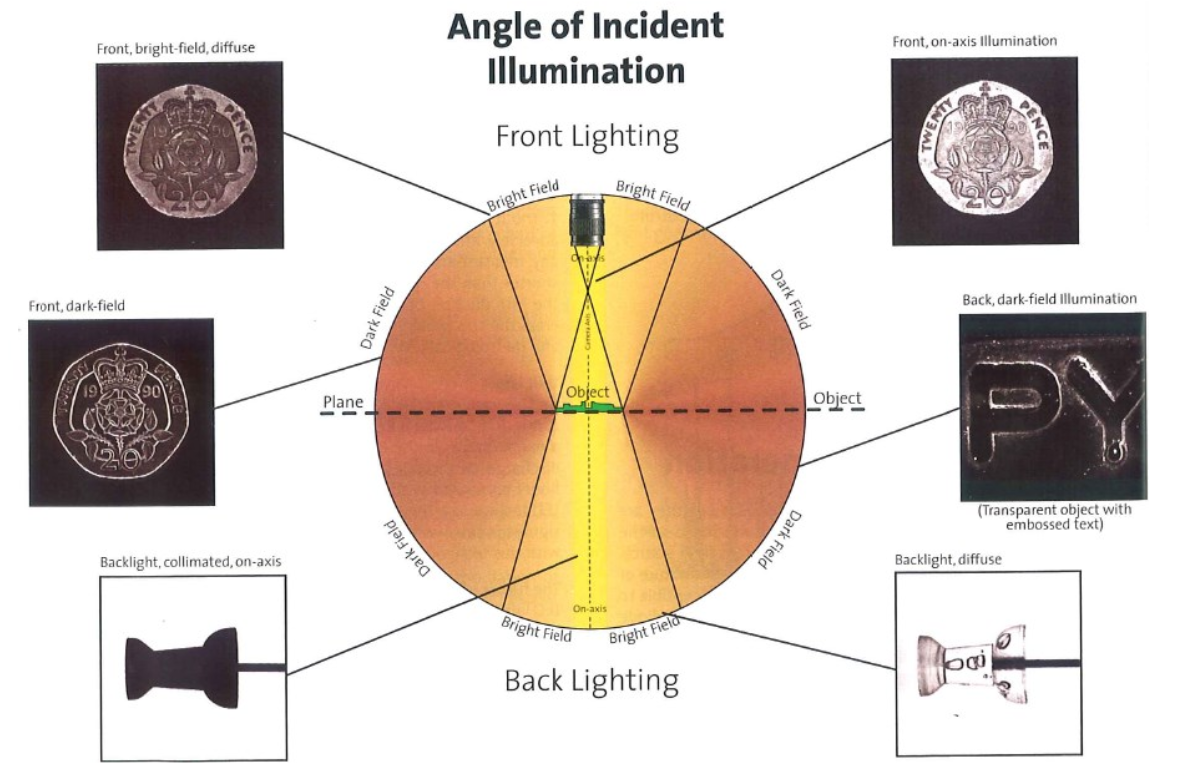
\includegraphics[width=0.8\columnwidth]{Images/02/Illumination.png}
    \caption{Angle of Incidence}
    \label{fig:02_Illumination}
\end{figure}
\subsection{Image Formation: Optics and Cameras}
\begin{itemize}
    \item Field of View (FoV): Area covered by the camera frame
    \item Working Distance (WD): Distance between camera focal point and object
    \item Resolution: The minimum feature size of the object that the imaging system can distinguish.
    \item Depth of Field (DOF): The range of distance photograph where objects appear sharp and in focus.
    \item Sensor Size: The size of a camera sensor's active area
    \item PMAG: The Primary Magnification of the lens is the ratio between the sensor size and the FOV.
\end{itemize}

\subsection{2D imahes as a discrete function}
Image Size / Sampling:
\begin{itemize}
    \item  M (rows) * N (columns) pixels (picture
    elements)
    \item Spatial resolution:
    \begin{itemize}
        \item size in the real world (e.g. dpi, lpi, pixel/m, …)
    \end{itemize}
    \item Coordinate system:
    \begin{itemize}
        \item origin in upper left corner,
        \item x-axis downwards, y-axis to the right!
    \end{itemize}
\end{itemize}
Quantization: Number of intensity values:
\begin{itemize}
    \item e.g 8 bit (256 values)
    \item Int:{0(black), 255(white)} or Double:{0.0(black), 1.0(white)}
\end{itemize}
	\section{Point Operations}
Homogeneous Point Operations(HPO)[Position independent]:
\[
I'(x,y) = f(I(x,y))
\]
Inhomogeneous Point Operations(IHPO)[Position dependent]:
\[
I'(x,y) = f(I(x,y),x,y)
\]
\subsection{Homogeneous Point Operations(HPO)}
\textbf{Properties:}
\begin{itemize}
    \item Global Operations
    \item fast, able to perform in real-time
    \item basically look up tables, constant performance time
\end{itemize}
\textbf{Thresholding:}
\[
f_{thresh}(a) =
\begin{cases}
    a_0 & \text{for } a < a_{th} \\
    a_1 & \text{for } a \geq a_{th}
\end{cases}
\]
\textbf{Invert:}
\[
f_{inv}(a) = a_{max} - a
\]
\textbf{Increase Brightness:}
\[
f_{bright}(a) = a + b
\]
\textbf{Increase Contrast:}
\[
f_{contrast}(a) = a \cdot c
\]
Limit Results by clamping: \( a' = \max(0,\min(a,255))\)

\textbf{Automatic Contrast Adjustment:}
\[
f_{ac} = a_{min} + (a - a_{low})    \cdot 
    \frac{a_{max} - a_{min}}{a_{high} - a_{low}} 
\]

\textbf{Modified Auto-Contrast:}
saturate \(\text{s}_\text{low}\) [\%] and \(\text{s}_\text{high}\)  [\%] pixel values.
\[
\hat{a}_{\text{low}} = \min \left\{ i \mid \mathrm{H}(i) \geq M \cdot N \cdot s_{\text{low}} \right\}
\]
\[
\hat{a}_{\text{high}} = \max \left\{ i \mid \mathrm{H}(i) \leq M \cdot N \cdot (1 - s_{\text{high}}) \right\}
\]
\[
f_{\text{mac}}(a) = 
\begin{cases}
a_{\min} & \text{for } a \leq \hat{a}_{\text{low}} \\
a_{\min} + (a - \hat{a}_{\text{low}}) \cdot \dfrac{a_{\max} - a_{\min}}{\hat{a}_{\text{high}} - \hat{a}_{\text{low}}} & \text{for } \hat{a}_{\text{low}} < a < \hat{a}_{\text{high}} \\
a_{\max} & \text{for } a \geq \hat{a}_{\text{high}}
\end{cases}
\]

\textbf{Gamma Correction:}
Compensate for the transfer characteristic of cameras, monitors, printers.
\[
f_{\gamma}(a) = a^{\bar{\gamma}} \quad \text{with } \bar{\gamma} = \frac{1}{\gamma} > 0
\]

\textbf{Histogram Equalization:} Adjusts image intensities so that the output histogram is approximately uniform, enhancing contrast by redistributing pixel values based on the cumulative histogram.
\textbf{Histogram Specification / Matching:} Generalization of Histogram Equalization. Match histogram to an arbitrary intensity distribution (e.g., of a reference image)

\subsection{Inhomogeneous Point Operations(IPO)}
\textbf{Shading Correctiom:}
\[
f_{\text{shading}}(a,x,y) = \frac{a}{s(x,y)} \quad s(x,y) = \text{shading function}
\]
\subsection{Others}
\begin{itemize}
    \item Bollean Operations(Masks)
    \item Arithmetic Operations
\end{itemize}
\subsection{Colour Spaces}
\textbf{RGB:}
\begin{itemize}
    \item Each Color component is on one axis
    \item Coordinate axes are perpendicular
    \item Pixels along the cube diagonal are grey values
\end{itemize}
\textbf{CMYK} (Cyan, Magenta, Yellow, and Key (Black))

\textbf{HSI} (Hue, Saturation, Intensity)

\textbf{HSL} (Hue, Saturation, Lightness)
	\section{Spatial Filtering}
Convolution and Correlation.
\subsection{Linear Filters}
\textbf{Mean Filter}:
\[
f_{mean}(I(u, v)) = \frac{1}{(2r+1)^2} \sum_{i=-r}^{r} \sum_{j=-r}^{r} I(u+i, v+j)
\]
where \(r\) is the radius of the filter kernel.
\subsubsection{Filter for Image Smoothing}
\textbf{Box Filter}:
\[
f_{box}(I(u, v)) = \frac{1}{(2r+1)^2} \sum_{i=-r}^{r} \sum_{j=-r}^{r} I(u+i, v+j)
\]
\textbf{Gaussian Filter}:
\[
f_{gauss}(I(u, v)) = \frac{1}{2\pi\sigma^2} \sum_{i=-r}^{r} \sum_{j=-r}^{r} I(u+i, v+j) \cdot e^{-\frac{i^2 + j^2}{2\sigma^2}}
\]
where \(\sigma\) is the standard deviation of the Gaussian distribution.

\subsection{Border Problems (Padding)}
Extend pixel values at the border (padding):
\begin{itemize}
    \item constant value, default is black (0)
    \item replicate pixels
    \item replicate cyclic 
\end{itemize}
\subsection{Non-Linear Filters}
All filters which use more than additions and multiplications.
\subsubsection{Rank Filters}
\textbf{Median Filter}:
\[
f_{median}(I(u, v)) = \text{median} \left( I(u+i, v+j) \right) \quad \text{for } i,j \in [-r,r]
\]

\textbf{Minimum Filter}:
\[
f_{min}(I(u, v)) = \min \left( I(u+i, v+j) \right) \quad \text{for } i,j \in [-r,r]
\]

\textbf{Maximum Filter}:
\[
f_{max}(I(u, v)) = \max \left( I(u+i, v+j) \right) \quad \text{for } i,j \in [-r,r] 
\]
\subsection{Difference Filters / Gradient Filters}
Linear filters with negative coefficients allow to pronounce edges and contours.

\textbf{Gradient Computation}: \(\frac{\partial f}{\partial u}(u) = \frac{f(u+1) - f(u-1)}{2}\)
 results in Kernel \(K = \left[-0.5\quad 0\quad 0.5\right]\)

\textbf{Filter for Edge Detection}:
\begin{itemize}
    \item Prewitt-Operator
    \item Sobel-Operator
    \item Compass Edge Filter
\end{itemize}

	\section{Frequency Domain Filtering}
Applications:
\begin{itemize}
    \item Linear Filters: Low-pass, High-pass, Band-pass
    \item Pattern detection (including noise removal)
    \item Image compression
    \item Inverse filtering for image restoration
\end{itemize}
\textbf{DFT for images(2D):}
\[
F(u,v) =\frac{1}{\sqrt{B\cdot H}} \sum_{x=0}^{B-1} \sum_{y=0}^{H-1} f(x,y)
\cdot
e^{-j2\pi\left(\frac{ux}{B} + \frac{vy}{H}\right)}
\]
\[
0 \leq u < B
\quad
0 \leq v < H
\]

Resulting Image in frequency domain has to be centered.

The phase contains important information!
\subsection{Applications of the DFT for images}
\textbf{Convolution Theorem:}
\[
f(x,y) * g(x,y) = \mathcal{F}^{-1}\left\{\mathcal{F}\{f(x,y)\} \cdot \mathcal{F}\{g(x,y)\}\right\}
\]
\begin{itemize}
    \item Operations are computationally cheaper in the frequency domain.
    \item All linear operations (high-pass, low-pass and band-pass) achieve high quality results and require less computational operations.
    \item Recognition and manipulation of periodic structures.
\end{itemize}
In order to use the DFT the origin of the kernel and the origin of the image
have to correspond.
\subsection{Periodic Noise Removal}
Suppressing the sine noise by switching off frequencies
	\section{Morphology}
Mostly used on binary images (can be used on gray level images as well)
\subsection{Binary Morphology}
First threshold image to binary image.
\textbf{Set Operations}:
\[
\begin{array}{rl}
\emptyset & \text{empty set} \\
A \subseteq B & A \text{ is part of } B \\
A \cap B & \text{intersection of } A \text{ and } B \text{: and} \\
A \cup B & \text{union of } A \text{ and } B \text{: or} \\
A^c & \text{complement } A \text{: not} \\
A - B & A \cap B^c : a \in A, a \notin B \\
A_z & A \text{ displaced by } z \text{ pixels: } a \in A : a_x + z_x, a_y + z_y \\
\hat{B} & B \text{ mirrored (point symmetry)}
\end{array}
\]
\subsection{Binary Morphology Operations}
2 basic operations:
\begin{itemize}
    \item Erosion: Eliminates small foreground structures, Shrinks foreground objects
    \[
    f_{erosion}(I) = I \ominus B = \{z \in \mathbb{Z}^2 | B_z \subseteq I\}
    \]
    \item Dilation: Small gaps in foreground structure are filled, Shrinks background objects
    \[
f_{dilation}(I) = I \oplus B = \{z \in \mathbb{Z}^2 | B_z \cap I \neq \emptyset\}
\]
\end{itemize}

Dilation and erosion are dual, i.e. one can be expressed in
terms of the other operation.
\subsection{Compound Operations}
\textbf{Opening}:
\[
f_{open}(I) = (I \ominus B) \oplus B
\]
\begin{itemize}
    \item Erosion followed by a dilation with the same structuring element
    \item Foreground structures smaller than H will be removed (Erosion)
    \item Dilation smooths the remaining structures and let them grow to their original size
\end{itemize}

\textbf{Closing}:
\[
f_{close}(I) = (I \oplus B) \ominus B
\]
\begin{itemize}
    \item Dilation followed by an erosion with the same structuring element
    \item Holes in foreground structures and small gaps smaller than the structuring element are filled
    \item Erosion let the remaining structure grow to its original size
\end{itemize}

\textbf{Boundary Extraction}:
\[
f_{boundary}(I) = I  - (I \ominus B)
\]
Size of B defines the thickness of the border.

\textbf{Hit-or-Miss Transform}:
\[
f_{hit-or-miss}(I)= I \ostar B_{1,2} = (I \ominus B_1) \cap (I^c \ominus B_2)
\]
\begin{itemize}
    \item Basic tool for shape detection and shape extraction
    \item \(B_1\) must be contained in foreground (hit in foreground)
    \item \(B_2\) must be contained in background (hit in background, miss in foreground)
\end{itemize}

\subsection{Applications}
\begin{itemize}
    \item Convex Hull
    \item Thinning
    \item Skeletons
    \item Pruning
\end{itemize}

\subsection{Grayscale Morphology}
2 kind of structuring elements:
\begin{itemize}
    \item Flat: All pixels have the same weight
    \item Non-flat: Pixels have different weights
\end{itemize}
\textbf{Grayscale Erosion}:
\[
[I \ominus b](x, y) = \min_{(s, t) \in b} \left\{ I(x + s, y + t) - b(s, t) \right\}
\]

\textbf{Grayscale Dilation}:
\[
[I \oplus b](x, y) = \max_{(s, t) \in \hat{b}} \left\{ I(x - s, y - t) + \hat{b}(s, t) \right\}
\]

\textbf{Opening / Closing (with flat structuring element)}

Opening: supresses bright details

Closing: supresses dark details

\subsection{Top Hat/Bottom Hat - Transformation}
\textbf{Top Hat}:
\[
f_{top-hat}(I) = I - (I \ominus B)
\]
Removes light objects on a dark background.

\textbf{Bottom Hat}:
\[
f_{bottom-hat}(I) = (I \oplus B) - I
\]
Removes dark objects on a bright
background
	\section{Image Coordinates}
\subsection{Image Coordinate System}
Sensor Coordinates:
\begin{itemize}
    \item The pixel-based, discrete coordinate system used in digital images.
    \item Origin: Top-left corner of the image.
    \item coordinates increasing to the right (x+-axis) and downward (y+-axis)
    \item \(u \rightarrow x, v \rightarrow y\)
\end{itemize}
Metric Cartesian Coordinates:
\begin{itemize}
    \item Continuous coordinate system used in image processing.
    \item Origin: Center of the image.
\end{itemize}

Camera Coordinate Systems:
\begin{figure}[ht]
    \centering
    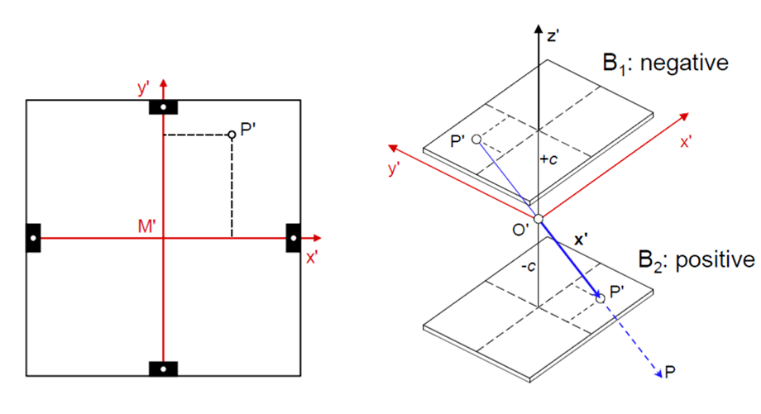
\includegraphics[width = \columnwidth]{Images/08/CameraCoordinateSystems.png}
    \caption{Camera Coordinate System}
    \label{fig:camera_coordinate_system}
\end{figure}
Paramters:
\begin{itemize}
    \item Image coordinate system origin (M', H', O')
    \item Camera constant c
\end{itemize}
are basic intrinsic camera parameters or
camera-intrinsics
\subsection{Transformation between Sensor and Cartesian Coordinates}
\[
x' = -\frac{s_x}{2} + \Delta x_s \cdot u
\]
\[
y' = \frac{s_y}{2} - \Delta y_s \cdot v
\]
Formulae implies the origin of the Cartesian coordinate system at the middle of the sensor \(\rightarrow\) That is rarely correct.

\subsection{Pinhole Camera: Approximation of an imperfect system!}
Physical camera is affected by a variety of error sources:
\begin{itemize}
    \item Lens distortion
    \item Non-planar sensor surface
    \item Temperature effects
\end{itemize}
Intrinsic parameters are computed through the camera calibration procedure.

\subsection{Homogeneous Coordinates}
\begin{itemize}
    \item \(K\): Camera matrix
    \item \(R\): Rotation matrix(orthonormal)
    \item \(t\): Translation vector
    \item \(\mathbf{x}\): Homogeneous image coordinates
    \item \(\mathbf{X}_{world}\): World coordinates
\end{itemize}
\[
\mathbf{x} = K \cdot [R | t] \cdot \mathbf{X}_{world}
\]


\[
\mathbf{x}_h =
\begin{bmatrix}
x_h \\
y_h \\
z_h \\
w
\end{bmatrix}
\qquad
\mathbf{x} =
\begin{bmatrix}
x_h / w \\
y_h / w \\
z_h / w \\
w / w
\end{bmatrix}
=
\begin{bmatrix}
x \\
y \\
z \\
1
\end{bmatrix}
\]

\[
\mathbf{X} =\mathbf{T}\cdot \mathbf{x}
\]
\[
\mathbf{T} =
\left[
\begin{array}{ccc|c}
a_{11} & a_{12} & a_{13} & a_{14} \\
a_{21} & a_{22} & a_{23} & a_{24} \\
a_{31} & a_{32} & a_{33} & a_{34} \\
\hline
a_{41} & a_{42} & a_{43} & a_{44}
\end{array}
\right]
=
\begin{bmatrix}
\mathbf{T}_{11} & \mathbf{T}_{12} \\
\mathbf{T}_{21} & \mathbf{T}_{22}
\end{bmatrix}
\]
\[
\begin{array}{rl}
\mathbf{T}_{11} : & \text{scaling, reflection in a line, rotation} \\
\mathbf{T}_{12} : & \text{translation} \\
\mathbf{T}_{21} : & \text{perspective} \\
\mathbf{T}_{22} : & \text{homogeneous scaling (factor } w\text{)}
\end{array}
\]
For exact matrices (for scale, rotation) see Presentation slides.
\subsection{Basic coordinate systems and the operations on them}
\textbf{Rigid registration = Similarity transformation}
\[
\mathbf{X} = \mathbf{A} \cdot \mathbf{x} + \mathbf{a}
\]
\[
\mathbf{X} = m \cdot \mathbf{R} \cdot \mathbf{x} + \mathbf{X}_0
\]
with 
\[
\mathbf{R} =
\begin{bmatrix}
\cos(\alpha) & -\sin(\alpha) \\
\sin(\alpha) & \cos(\alpha) \\
\end{bmatrix}
\]
\textbf{Polynomial Transformation}
\[
X = \sum_{j=0}^{n} \sum_{i=0}^{j} a_{ji} \cdot x^{j-i} \cdot y^{i}
\]

\[
Y = \sum_{j=0}^{n} \sum_{i=0}^{j} b_{ji} \cdot x^{j-i} \cdot y^{i}
\]

\subsubsection{Projective Transformation}
3D Space to Plane Mapping

\textbf{Central Projection:}

\[
X = \frac{a_0 + a_1 \cdot x + a_2 \cdot y}{1 + c_1 \cdot x + c_2 \cdot y}
\]

\[
Y = \frac{b_0 + b_1 \cdot x + b_2 \cdot y}{1 + c_1 \cdot x + c_2 \cdot y}
\]

\[
a_0 + a_1 x + a_2 y - X - c_1 x X - c_2 y X = 0
\]

\[
b_0 + b_1 x + b_2 y - Y - c_1 x Y - c_2 y Y = 0
\]
\textbf{Homography:} Plane to Plane transformation
\[
\begin{bmatrix}
x_2 \\
y_2 \\
z_2
\end{bmatrix}
=
\begin{bmatrix}
H_{11} & H_{12} & H_{13} \\
H_{21} & H_{22} & H_{23} \\
H_{31} & H_{32} & H_{33}
\end{bmatrix}
\begin{bmatrix}
x_1 \\
y_1 \\
z_1
\end{bmatrix}
\quad \Leftrightarrow \quad
\mathbf{x}_2 = H \mathbf{x}_1
\]
with \(x'_2 = x_2/z_2\) and \(y'_2 = y_2/z_2\)

\[
x'_2 = \frac{H_{11}x_1 + H_{12}y_1 + H_{13}z_1}{H_{31}x_1 + H_{32}y_1 + H_{33}z_1}
\]

\[
y'_2 = \frac{H_{21}x_1 + H_{22}y_1 + H_{23}z_1}{H_{31}x_1 + H_{32}y_1 + H_{33}z_1}
\]
Create 4 equation pairs to solve projection problem using eigenvalue decomposition…
\subsection{Overview Transformations}
Isometric Transformation:
\[
\mathbf{x}' = 
\begin{pmatrix}
R & \mathbf{t} \\
\mathbf{0}^\mathrm{T} & 1
\end{pmatrix}
\mathbf{x}
\]

Similarity Transformation:
\[
\mathbf{x}' = 
\begin{pmatrix}
sR & \mathbf{t} \\
\mathbf{0}^\mathrm{T} & 1
\end{pmatrix}
\mathbf{x}
\]
Affine Transformation:
\[
\mathbf{x}' = 
\begin{pmatrix}
A & \mathbf{t} \\
\mathbf{0}^\mathrm{T} & 1
\end{pmatrix}
\mathbf{x}
\]

\[
A = R(\theta) R(-\phi) D R(\phi)
\]

\[
D = 
\begin{pmatrix}
\lambda_1 & 0 \\
0 & \lambda_2
\end{pmatrix}
\]
Homography:

\[
\mathbf{x}' = 
\begin{pmatrix}
A & \mathbf{t} \\
\mathbf{v}^\mathrm{T} & v
\end{pmatrix}
\mathbf{x}
\]

\subsection{Distortions}
All effects are caused by different aperture
positions.
\begin{itemize}
    \item Barrel distortion effect
    \item Cushion distortion effect
\end{itemize}

\subsubsection{Chromatic abberation (Color Error)}
\begin{itemize}
    \item Causes the bias in the data
    \item Causes problems by object recognition
    \item Changes in different lightconditions
\end{itemize}


\end{document}
